\subsection{Consideraciones generales}
Para armar los circuitos propuestos por la cátedra se dispone de un
amplificador operacional LM-833N. Los datos más importantes a considerar
vistos en la hoja de datos son los siguientes:
\begin{enumerate}
    \item $A_{vol}$ = $110dB$
    \item BWP = $15 MHz$

\end{enumerate}    

\subsection{Circuito Derivador}
A continuación se realiza el análisis sobre el circuito derivador planteado
por la cátedra utilzando un amplificador operancional $LM833$ propuestado por 
la cátedra en el siguiente circuito.
\begin{figure}[H]
    \centering
    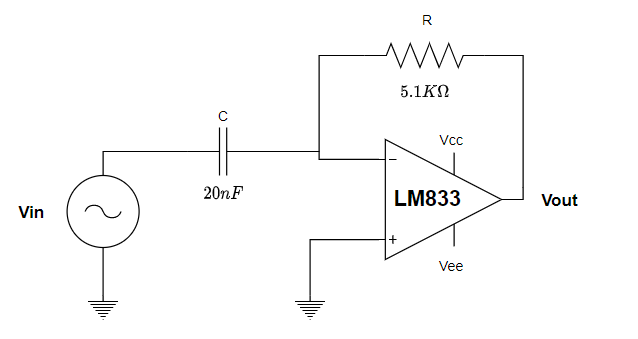
\includegraphics[width=0.6\textwidth]{../Ejercicio3-CircuitoIntegradoresyDerivadores/Imagenes/circuito_derivador.png}
    \caption{Circuito derivador implementado con Opamp}
\end{figure}

Consiguientemente, se procede a calcular la transferencia de tensión entra
la entrada y salida del circuito. \par 
En condición ideales se puede se considera que la ganancia del
amplificador operacional es infinita por lo que, basándonos en 
su ecuación característica (\ref{eq_opamp}), se puede asegurar que para 
mantener la relación $V^+=V^-$ van a tender a 0.
\vspace{2mm}
\begin{equation*}
    V_{out}=A_0(V^+-V^-)
    \label{eq_opamp}
\end{equation*}
\vspace{2mm}
Por lo tanto, se pueden escribir a las corrientes del circuito como:
\vspace{2mm}
\begin{equation*}
    I_1=\frac{V{in}}{X_c}=V_{in}\$C_1 \indent \indent I_2=\frac{V_{out}}{R}
    \label{eq_avol_ideal}
\end{equation*}
\vspace{2mm}
Considerando que $V^-=0$ y que $I_1=I_2$ se logra llegar a la transferencia bajo 
condiciones ideales:
\vspace{2mm}
\begin{equation}
    H(\$)=\frac{V_{out}}{V_{in}}=-R\$C
    \label{trans_ideal}
\end{equation}
\vspace{2mm}
Por otro lado, considerando a $A_{vol}$ finito se vuelve indispensable reformular las
ecuaciones vistas en \ref{eq_avol_ideal} ya que al considerar un $A_vol$ que no 
tiende a infinito se vuelve imposible asegurar que la tensión $V^-$ sea nula. Bajo 
las nuevas circunstancias se obtienen:
\vspace{2mm}
\begin{equation*}
    I_1=\frac{V{in}-V^-}{X_c}=(V_{in}-V^-)\$C_1 \indent \indent I_2=\frac{V_{out}-V^-}{R}
    \label{eq_avol_noideal}
\end{equation*}
\vspace{2mm}
Utilizando \ref{eq_opamp} y \ref{eq_avol_noideal} se puede despejar la transferencia
como:
\vspace{2mm}
\begin{equation}
    H_1(\$)=\frac{V_{out}}{V_{in}}=\frac{-R\$C}{1+(\frac{R\$C+1}{A_0})}
    \label{trans_no_ideal}
\end{equation}
\vspace{2mm}
Se puede validar este ecuación considerando:
 $$\lim_{A_0\to\infty} H_1(\$)$$
Se obtiene la transferencia en condiciones ideales vista en \ref{trans_ideal}. \par
Para finalizar se realiza un análisis considerando $A_{vol}$ variante en frecuencia
debido a la presencia de un polo dominante que le da una respuesta en frecuencia 
característica de un filtro pasa-bajos. La dependencia en frecuencia de la ganancia
del opamp está dada por la siguiente fórmula:
\vspace{2mm}
\begin{equation}
    A_v(\$)=\frac{A_0}{1+\frac{\$}{w_b}}
    \label{a_vol_frec}
\end{equation}
\vspace{2mm}
Siendo $A_0$ la ganancia en continua y $w_b$ el ancho de banda del filtro,
 la frecuencia para la cual el dispositivo atenúa 3 dB. \par 
 Reemplazando (\ref{a_vol_frec}) en (\ref{trans_no_ideal}) se obtiene:
 \vspace{2mm}
 \begin{equation}
    H_2(\$)=\frac{-R\$C}{1+\frac{1}{A_0}+\frac{R\$C}{A_0}+\frac{R\$^2C}{w_bA_0}}
    \label{trans_frec}
\end{equation}
\vspace{2mm}
Esta ecuación se puede dividir según su ganancia ideal $G_I$ y su factor de corrección
$F_c$ de la siguiente forma:
\vspace{2mm}
\begin{equation*}
   G_I=-R\$C \indent \indent F_c=\frac{1}{1+\frac{1}{A_0}+\frac{R\$C}{A_0}+\frac{R\$^2C}{w_bA_0}}
   \label{trans_frec}
\end{equation*}
\vspace{2mm}
Siguiendo el mismo procedimiento aplicado para $H_1(\$)$, se puede 
 $$\lim_{A_0\to\infty} H_2(\$)=\lim_{A_0\to\infty} G_IF_C=G_I=H(\$)$$

Las expresiones obtenidas se plasman en el siguiente gráfico, pudiéndose 
observar una mayor precisión a medida que se usan modelos más realistas
sin consideraciones ideales.
\begin{figure}[H]
    \centering
    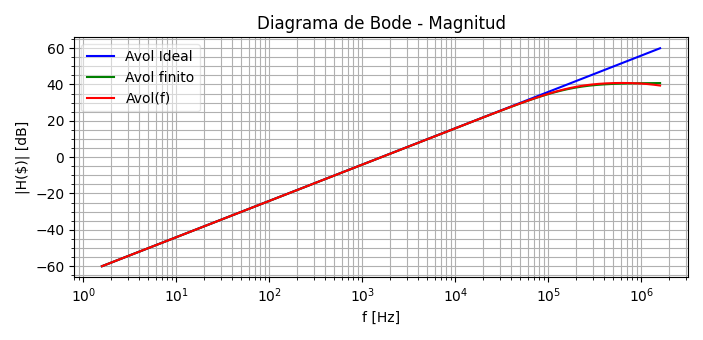
\includegraphics[width=0.6\textwidth]{../Ejercicio3-CircuitoIntegradoresyDerivadores/Imagenes/Derivador/bode_derivador magnitud.png}
    \caption{Respuesta en frecuencia teóricas - Modulo}
\end{figure}
\begin{figure}[H]
    \centering
    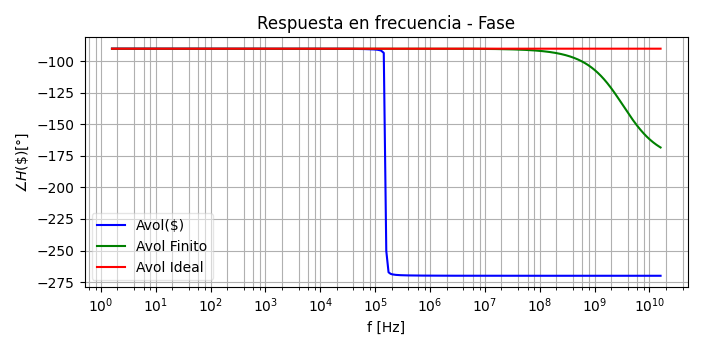
\includegraphics[width=0.6\textwidth]{../Ejercicio3-CircuitoIntegradoresyDerivadores/Imagenes/Derivador/bode_derivador_fase.png}
    \caption{Respuesta en frecuencia teóricas - Fase}
\end{figure}










